\chapter{Identificazione dei modelli}
L'identificazione di un modello matematico per un sistema biologico richiede un'attenta transizione dal sistema reale alla sua rappresentazione formale. Questo processo si articola tipicamente in due passaggi fondamentali: in primo luogo, è necessario definire la struttura matematica del modello (determinazione della struttura); in secondo luogo, occorre determinare quantitativamente tutti i parametri associati a tale struttura. Quest'ultima fase, che prende il nome di \textbf{identificazione}, unita al primo passo, fornisce il modello matematico nella sua forma completa.

\section{Raccolta Dati e Disegno Sperimentale}
Per poter risolvere il problema dell'identificazione e stimare i parametri del modello, il prerequisito fondamentale è la \textbf{disponibilità di dati}. In alcuni casi, i dati possono provenire dalle dinamiche intrinseche del sistema biologico stesso, come oscillazioni spontanee o rumore fisiologico di fondo. Tuttavia, più frequentemente è necessario intervenire in modo attivo definendo un apposito disegno sperimentale (\emph{experimental design}) finalizzato alla raccolta mirata dei dati. Un esperimento tipico consiste nell'applicare al sistema in esame specifici segnali di test (variabili di input) e registrarne l'evoluzione temporale della risposta (variabili di output).

\section{Selezione dei Segnali di Test}
La scelta dei segnali di eccitazione non è arbitraria, ma è guidata da specifici criteri tesi a massimizzare le informazioni raccolte preservando la natura del sistema:
\begin{itemize}
    \item \textbf{Fattibilità e adeguatezza:} I segnali di test devono essere convenienti da generare e adatti al sistema in esame. Esempi classici includono la somministrazione di un farmaco mediante iniezione in bolo per gli studi di farmacocinetica, o una variazione a gradino nella concentrazione di ossigeno inalato per studiare la dinamica del sistema respiratorio.
    \item \textbf{Ampiezza e vincoli di sicurezza:} I segnali devono essere il più ampi possibile al fine di produrre un output caratterizzato da un elevato rapporto segnale/rumore. Tuttavia, si scontrano con vincoli pratici inderogabili: occorre rispettare severe considerazioni etiche e di sicurezza sulla salute del paziente o del campione biologico. Inoltre, da un punto di vista sistemistico, il disturbo introdotto non deve allontanare il sistema dalla regione di linearità in cui il modello strutturale risulta valido.
    \item \textbf{Efficienza temporale:} Il segnale di test ideale deve minimizzare il tempo complessivo necessario allo svolgimento dell'esperimento e al successivo processo di identificazione.
\end{itemize}

In generale, i segnali di test impiegati nella pratica sperimentale si classificano in tre grandi categorie: segnali che producono una risposta transitoria, segnali che producono una risposta in frequenza (armonici) e segnali casuali.

\subsection{Segnali Transitori}
I segnali di test che producono una risposta transitoria sono quelli maggiormente impiegati, specialmente in ambiti come gli studi metabolici e la farmacocinetica. Le forme di input più usuali sono l'impulso (iniezione) e il gradino (un'infusione continua o variazione a gradino di gas). Una volta applicato l'ingresso, si osserva la risposta impulsiva o la risposta a gradino del sistema, che sono matematicamente legate tra loro.
\begin{figure}[h]
    \centering
    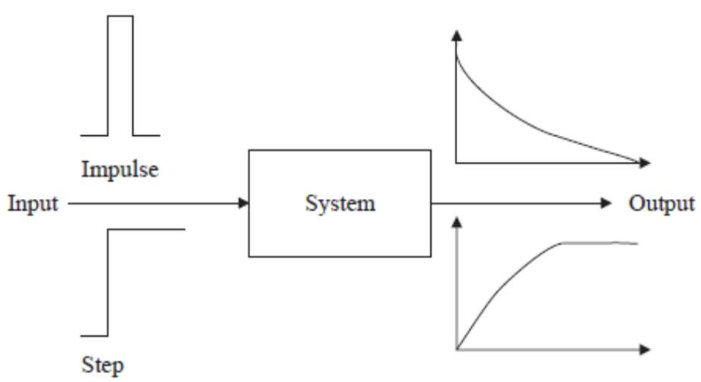
\includegraphics[width=0.5\linewidth]{immagini/segnali_di_test_transitori.png}
\end{figure}

Il test della risposta impulsiva presenta il vantaggio di essere proceduralmente semplice e di breve durata, in quanto l'interesse risiede unicamente nel comportamento transitorio e non nell'analisi delle dinamiche a regime. Ciononostante, presenta dei limiti pratici nell'applicazione:
\begin{enumerate}
    \item L'ampiezza dell'impulso rappresenta un compromesso delicato: se il segnale è troppo piccolo, provoca un'inadeguata eccitazione del sistema; se è eccessivamente grande, rischia di portare il sistema fuori dalla sua regione di validità lineare.
    \item Non vi è alcun filtraggio intrinseco del rumore; questo comporta che rumore ambientale o altri input non controllati possano generare un elevato errore sull'uscita registrata.
    \item Nelle applicazioni in vivo, vi è un numero ristretto di siti anatomici per la somministrazione e la frequenza di campionamento tramite prelievi è limitata, portando talvolta all'uso di tecniche di imaging come alternativa meno invasiva.
\end{enumerate}

\subsection{Segnali Armonici}
Il test della risposta in frequenza consiste nell'applicare segnali armonici (sinusoidi pure) a diverse frequenze e osservare gli effetti che il sistema produce sull'uscita, misurandone l'amplificazione (o attenuazione) e lo sfasamento. Se si considera un sistema lineare tempo-invariante (LTI), applicando in ingresso un segnale $A \sin(\omega t)$, l'uscita a regime sarà data da:
\[
y(t) = A |G(j\omega)| \sin(\omega t + \angle G(j\omega))
\]
dove $G(j\omega)$ è la funzione di trasferimento in frequenza del sistema.
\begin{figure}
    \centering
    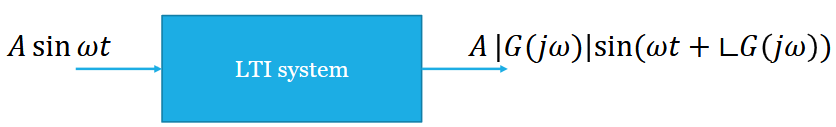
\includegraphics[width=0.7\linewidth]{immagini/segnali di test armonici.png}
\end{figure}
Pur essendo meno convenienti da applicare da un punto di vista pratico e richiedendo spesso strumentazione speciale (come analizzatori di spettro), i segnali armonici presentano notevoli vantaggi. Consentono di eccitare selettivamente tutti i modi del sistema senza dover somministrare segnali di ampiezza eccessiva. Garantiscono inoltre un ottimo filtraggio intrinseco del rumore, poiché l'analisi dell'uscita si concentra su una sola componente in frequenza alla volta. Un notevole svantaggio risiede nella lunga durata del test: ogni frequenza va testata singolarmente, ed è necessario un tempo di attesa sufficiente per far decadere gli effetti transitori iniziali in modo da misurare unicamente la componente a regime. I dati di risposta in frequenza raccolti possono poi essere impiegati per adattare (fittare) modelli parametrici al fine di stimare i parametri incogniti del sistema.

\subsection{Segnali Random}
I segnali random offrono una terza via molto interessante per l'identificazione. Consideriamo un sistema LTI con risposta impulsiva $g(t)$. Applicando in ingresso un segnale generico $m(t)$ e misurando l'uscita $y(t)$, si può dimostrare che la funzione di cross-correlazione tra l'ingresso e l'uscita, indicata con $R_{my}(\tau)$, è legata all'autocorrelazione dell'ingresso $R_{mm}$ e alla risposta impulsiva dalla seguente equazione integrale di convoluzione:
\[
R_{my}(\tau) = \int_{-\infty}^{\infty} g(t) R_{mm}(t-\tau) d\tau = g*R_{mm}
\]
Se come input si sceglie un segnale che approssima il \textbf{rumore bianco} (caratterizzato da uno spettro con densità di potenza costante a tutte le frequenze e da un'autocorrelazione impulsiva), la relazione si semplifica notevolmente, restituendo direttamente:
\[
R_{my}(\tau) = g(\tau)
\]
Il test prevede quindi l'applicazione di un segnale di tipo rumore bianco (nella pratica, spesso si usano sequenze binarie pseudo-random o PRBS) calcolando poi a posteriori la cross-correlazione per ricostruire la risposta impulsiva $g(t)$. 
Poiché un segnale casuale eccita lo spettro su tutte le frequenze, questo test equivale a eseguire test armonici multipli contemporaneamente, rendendolo concettualmente più rapido, seppur più oneroso sul piano computazionale. Il processo di integrazione necessario al calcolo della cross-correlazione funge da eccellente filtro per le componenti di rumore estranee. Va notato che, per assicurare l'accuratezza statistica della stima della cross-correlazione, il test deve comunque essere protratto per un intervallo di tempo sufficientemente lungo.
\newpage
\section{Sorgenti di Errore}
L'operazione di stima dei parametri è fisiologicamente affetta da diverse sorgenti di errore e rumore, inquadrabili nelle seguenti categorie:

\begin{wrapfigure}{r}{0.5\textwidth}
  \begin{center}
    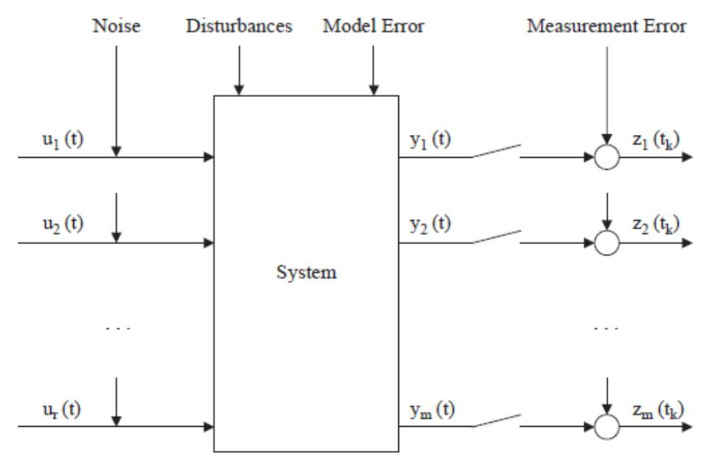
\includegraphics[width=0.5\textwidth]{immagini/sorgenti di errore.png}
  \end{center}
\end{wrapfigure}
\begin{itemize}
    \item \textbf{Imperfezioni del segnale di test:} L'input reale spesso si discosta dalla forma teorica ideale assunta matematicamente (ad esempio, un impulso non infinitamente stretto o un segnale random che non è un vero rumore bianco).
    \item \textbf{Errori di misura:} Rappresentano l'incertezza e il rumore della strumentazione sulle misurazioni delle variabili di uscita. 
    \item \textbf{Disturbi:} Fluttuazioni e interferenze da parte di altre variabili esterne al sistema.
    \item \textbf{Errore di modello:} Discrepanza sistematica tra la struttura formale postulata (la matematica) e la realtà del processo biologico sottostante.
\end{itemize}

Tra questi, l'\textbf{errore di misura} è l'unico che può essere modellato e trattato in maniera analiticamente rigorosa. Tradizionalmente, si assume un'ipotesi di additività dell'errore. Denotando con $z_l$ la misura campionata all'istante $t_i$, con $y_l$ l'uscita predetta dal modello per un dato vettore di parametri $p$, e con $v_l$ il termine di errore aleatorio, possiamo scrivere:
\begin{equation}
\begin{split}
    z_l(t_i, p) &= y_l(t_i, p) + v_l(t_i) \\ \text{per } i&=1,2,\dots,N_l \\ e \quad l&=1,2,\dots,m
\end{split}
\end{equation}
Per consentire algoritmi di identificazione robusti, è necessario fornire una caratterizzazione statistica adeguata di $v_l$ (ad esempio, ipotizzando una distribuzione gaussiana o poissoniana, rumore bianco, o scorrelato nel tempo). Quanto più precisa sarà questa caratterizzazione teorica, tanto minore sarà l'impatto negativo dell'errore sull'affidabilità della stima dei parametri. Se non avessimo errori di misura le nostre misure sarebbero deterministiche. 
\newpage
\section{Il Processo di Identificazione}
A livello concettuale, il problema complessivo dell'identificazione si biforca spesso in due tipologie distinte di analisi: la stima dei parametri e la stima dei segnali.

\subsection{Stima dei Parametri}
Prima di lanciare algoritmi per la stima numerica, occorre necessariamente verificare l'\textbf{identificabilità a priori} del modello. Questa analisi teorica risponde a una domanda fondamentale: indipendentemente dall'errore nei dati, ho misurato un numero sufficiente di variabili per poter stimare in maniera univoca tutti i parametri interni del modello strutturale? 

Nel caso in cui l'identificabilità non sia garantita (ad esempio, la stima risulta non univoca), si presentano due soluzioni pratiche:
\begin{enumerate}
    \item Ridurre la complessità e l'ordine del modello, abbassando il numero di parametri da stimare, avendo cura di validare se la versione semplificata rimane adeguata al contesto fisiologico.
    \item Aumentare la base di dati, aggiungendo un nuovo esperimento o iniziando a misurare un'ulteriore variabile di output precedentemente non osservata.
\end{enumerate}
Una volta che il sistema risulti a priori identificabile, si procede alla stima. Tra le tecniche più consolidate figurano gli approcci ai minimi quadrati (sia lineari che non lineari), i metodi basati sul principio della massima verosimiglianza (\emph{Maximum Likelihood}), e l'approccio probabilistico Bayesiano.

\subsection{Stima del Segnale}
Non sempre l'obiettivo è ricavare i parametri numerici (resistenza, costante di decadimento, ecc.) del sistema biologico. A volte, si intende stimare l'andamento di un segnale incognito. Tipicamente le relazioni analizzate mettono in gioco tre grandezze: il segnale di input, la risposta impulsiva del sistema, e il segnale di output misurato. 
Quando ne conosciamo due e vogliamo stimare la terza, applichiamo algoritmi focalizzati sui segnali (come ad esempio la \emph{deconvoluzione}, necessaria quando si intende risalire all'input originario conoscendo il sistema e l'uscita). Per gestire l'intrinseca instabilità di tali calcoli, si fa spesso ricorso a tecniche matematiche avanzate note come algoritmi di \emph{regolarizzazione}.